%%%% methodologie_donnees_boussole.tex
%%%% Data Challenge Burkina 2026, édition Éducation, défi 3 : méthodologie de collecte et de nettoyage
%%%% Mise en page reprise du gabarit de la note d'intention.
%%%% Évaluation anonyme : ne mettre aucun nom, aucune affiliation, aucun lien personnel.

\documentclass{article}
\pdfpagewidth=8.5in
\pdfpageheight=11in

\usepackage{ijcai26}

\usepackage{times}
\usepackage{url}
\usepackage[utf8]{inputenc}
\usepackage[T1]{fontenc}
\usepackage[english,french]{babel}
\usepackage{xcolor}
\usepackage{xurl}
\usepackage[colorlinks=true,
            citecolor=blue!70!black,
            linkcolor=red!60!black,
            urlcolor=blue!70!black,
            pdfauthor={},
            pdftitle={Boussole Scolaire : méthodologie de collecte et de nettoyage des données},
            pdfcreator={},
            pdfproducer={}]{hyperref}
\usepackage[small]{caption}
\usepackage{graphicx}
\usepackage{amsmath}
\usepackage{booktabs}
\usepackage{tabularx}
\usepackage{array}
\usepackage{float}
\usepackage{placeins}

\urlstyle{same}
\emergencystretch=1.5em
\graphicspath{{figures/}}

\addto\captionsfrench{%
  \renewcommand{\tablename}{Tableau}%
  \renewcommand{\figurename}{Figure}%
  \renewcommand{\refname}{Références}%
}

\newcommand{\sol}{Boussole Scolaire}
\newcolumntype{L}[1]{>{\raggedright\arraybackslash}p{#1}}
\newcolumntype{Y}{>{\raggedright\arraybackslash}X}

\pdfinfo{
/TemplateVersion (IJCAI.2026.0)
}

\title{\sol{}\\[3pt]
{\large\mdseries Méthodologie de collecte et de nettoyage des données}}
\author{
Data Challenge Burkina 2026, édition Éducation, défi 3\\
\affiliations
Documentation technique, étapes 01 (collecte) et 02 (nettoyage)
}

\begin{document}
\renewcommand{\tablename}{Tableau}\renewcommand{\figurename}{Figure}\renewcommand{\refname}{Références}
\raggedbottom

\maketitle
\thispagestyle{plain}
\pagestyle{plain}

%======================================================================
\section{Objet}
%======================================================================

\sol{} prévoit la demande scolaire de la rentrée et aide à répartir les enseignants et les salles de classe là où ils réduisent le plus les inégalités d'encadrement. Ce document décrit les deux premières étapes du parcours des données fixé par le challenge~\cite{dcb_document} : la collecte, qui rassemble sans les modifier les données utiles au défi, et le nettoyage, qui les transforme en une base unique et contrôlée. Il précise les fichiers exploités et écartés, les règles appliquées, les contrôles et les limites.

Trois règles encadrent le travail. Seules les données remises par les organisateurs sont utilisées : la base principale de la DGESS~\cite{dgess_base} et le Data Pack~\cite{dcb_guide}. Ces fichiers ne sont jamais modifiés : le code refuse d'écrire dans le Data Pack, la base principale et le document du challenge. Enfin, chaque valeur garde la trace de son fichier, de sa page et de sa ligne d'origine, et toute la chaîne se relance par une commande.

%======================================================================
\section{Des données choisies pour l'offre et la demande}
%======================================================================

Le défi porte sur l'offre scolaire (enseignants, écoles, salles) confrontée à la demande (élèves, présents et à venir), dans un contexte de crise sécuritaire qui ferme et rouvre des écoles. Les sources ont été choisies selon ces trois questions (tableau~\ref{tab:sources}).

\begin{table*}[!t]
\centering
\small
\begin{tabularx}{\textwidth}{@{}L{2.4cm} L{4.2cm} Y L{2.3cm} L{2.2cm}@{}}
\toprule
Question & Source & Contenu retenu & Niveau & Période \\
\midrule
Quelle est l'offre ? & Annuaires du primaire DGESS (8 éditions)~\cite{dgess_annuaires} & Écoles, salles, groupes pédagogiques, maîtres (I.1) ; enseignants par corps, fonction, âge et ancienneté (IV) ; écoles par statut, taille, équipement (V) ; année de mise en service, logements de maître, nature et état des murs et des toitures (VI) & Province & 2017-2018 à 2024-2025 \\
 & Annuaires statistiques régionaux INSD 2024~\cite{insd_regionaux} & Écoles, salles, salles sous paillote, élèves, enseignants & Commune (10 régions sur 13) & Environ 2014 à 2024 \\
 & Annuaires statistiques nationaux INSD~\cite{insd_regionaux} & Pages sur les écoles, salles et enseignants du primaire ; édition 2024 en 17 régions & Région & 2015 à 2024 \\
 & Tableaux de bord DGESS~\cite{dgess_tdb} & Séries régionales des ratios d'encadrement & Région & 2015-2016 à 2023-2024 \\
Quelle sera la demande ? & Annuaires DGESS (VIII, III.7) & Historique des effectifs et des redoublants par niveau ; nouveaux entrants au CP1 par âge & Province & Une dizaine d'années par édition \\
 & RGPH 2019 et projections~\cite{insd_rgph} & Population par commune et par localité ; population projetée 2020-2035 & Commune, localité, région & 2019 à 2035 \\
 & Base principale DGESS~\cite{dgess_base} & Effectifs, admission, scolarisation, écoles & Région & 2015-2016 à 2024-2025 \\
Dans quel contexte ? & Rapports mensuels ST-ESU~\cite{stesu} & Écoles fermées, rouvertes et délocalisées ; élèves et enseignants touchés & Région, province & Nov. 2021 à fév. 2026 \\
 & Déplacés internes CONASUR~\cite{conasur} & Déplacés accueillis, dont enfants & Commune & 2019 à 2025 \\
 & COD-AB~\cite{codab} et OpenStreetMap~\cite{hotosm} & Communes avec ancien et nouveau code ; écoles géolocalisées & Commune, point & 2025, 2026 \\
\bottomrule
\end{tabularx}
\caption{Sources retenues pour \sol{}. Source : fichiers remis par les organisateurs ; classement des auteurs.}
\label{tab:sources}
\end{table*}

Sur les 173 fichiers sources remis, 88 sont retenus et répartis en 26 sources, et 85 sont écartés pour un motif écrit (tableau~\ref{tab:ecartes}). Aucun fichier n'est resté sans décision. Les conditions de vie, la pauvreté et la santé, utiles pour comprendre la demande, n'entrent pas dans la répartition de l'offre et sont écartées. Les annuaires des ONG ont été examinés : ils ne contiennent aucun tableau propre à l'éducation.

\begin{table}[!t]
\centering
\small
\begin{tabularx}{\columnwidth}{@{}Y r@{}}
\toprule
Motif d'exclusion & Fichiers \\
\midrule
Éducation non formelle, préscolaire & 28 \\
Conditions de vie, pauvreté, santé, emploi & 14 \\
Synthèses et dépliants, redondants avec les annuaires & 12 \\
Géométries et métadonnées cartographiques & 9 \\
Résultats généraux et documentation du RGPH & 10 \\
Post-primaire, secondaire, supérieur & 3 \\
Documentation du challenge et du Data Pack & 5 \\
Annuaires des ONG, séries nationales, doublon des projections & 4 \\
\midrule
Total & 85 \\
\bottomrule
\end{tabularx}
\caption{Fichiers écartés et motifs. Source : bilan des sources, calculs des auteurs.}
\label{tab:ecartes}
\end{table}

%======================================================================
\section{Méthode de collecte}
%======================================================================

\textbf{Des sources déclarées, pas programmées.} Les sources sont décrites dans un fichier de déclaration lisible sans programmation : pour chacune, les fichiers concernés, la règle de sélection des pages, l'usage prévu et le nom du dépôt. Les motifs d'exclusion des fichiers non retenus y figurent aussi. Ajouter une source ou en écarter une ne demande donc pas de modifier le code.

\textbf{Repérer les tableaux par leur titre de section.} Dans les annuaires, les numéros de page changent d'une édition à l'autre, mais chaque page porte en tête le titre de sa section, numéroté en chiffres romains et écrit en majuscules (« V.2 RÉPARTITION DES ÉCOLES ET SALLES DE CLASSES »). Une page est retenue si ce titre contient tous les mots-clés de la source. La table des matières, rédigée en minuscules, est écartée d'office. Pour les annuaires de l'INSD, dont la numérotation des tableaux varie d'une région à l'autre, la page est retenue si un titre de tableau associe le primaire et la commune ; les pages de suite sans titre sont rattachées au tableau qui précède.

\textbf{Tracer chaque fichier.} Chaque ligne copiée indique son fichier d'origine, son extraction CSV et sa période. Un registre décrit chaque fichier utilisé : pages extraites, nombre de lignes, empreinte SHA-256, producteur, adresse de téléchargement et date de collecte. Un contrôle de couverture vérifie que chaque section est trouvée dans chacune des huit éditions : les quatorze sections le sont, sans alerte.

\textbf{Résultat.} La collecte copie 247\,486 lignes issues de 204 fichiers, en deux minutes. Le dépôt 01 compte 30 fichiers nommés selon la convention du challenge, avec un LISEZ-MOI.

%======================================================================
\section{Méthode de nettoyage}
%======================================================================

\subsection{Les territoires}

Les annuaires suivent l'ancien découpage, en 13 régions et 45 provinces, alors que le pays compte 17 régions et 47 provinces depuis juillet 2025. Le référentiel COD-AB~\cite{codab} donne, pour chacune des 351 communes, son code actuel et son ancien code ; les noms des anciennes provinces et régions viennent du fichier des écoles OpenStreetMap~\cite{hotosm}. La base contient ainsi les communes, les 45 anciennes provinces (avec les provinces de 2025 qui en sont issues) et les 13 anciennes régions.

\textbf{Reconnaître les noms automatiquement.} Les noms des tableaux ne sont pas toujours écrits comme dans le référentiel. Chaque nom est rapproché d'un code en trois temps : égalité exacte après normalisation (majuscules, sans accent ni ponctuation), égalité après retrait d'un article en tête, puis orthographe la plus proche si la similarité dépasse 0,85. Chaque rapprochement non exact est consigné : « LES BALE » est reconnu comme la Balé, « KOMONDJARI » comme la Komandjari.

\subsection{Un lecteur unique pour les tableaux provinciaux}

Les tableaux provinciaux des annuaires partagent une même structure : un nom de région en titre de bloc, puis pour chaque province une ligne par statut (public, privé, total) et une ligne de total régional. Un lecteur unique, paramétré par le nombre de colonnes attendu et par les intertitres à suivre (par exemple « murs » ou « toitures », « public » ou « privé »), les transforme en tables longues, puis larges : une ligne par édition, province et statut. Les lignes de pourcentage, recalculables, et les numéros de page sont ignorés ; toute autre ligne inattendue est signalée.

\subsection{Les tables produites}

Huit tables de faits sont construites. La table de l'offre donne, pour chaque province, édition et statut, les écoles, les salles, les groupes pédagogiques, les maîtres chargés de cours et les élèves ; les élèves par maître, par salle et par groupe pédagogique en sont recalculés. La table de l'état des salles donne la nature et l'état des murs et des toitures, et la part des salles précaires. La table des enseignants donne, par sexe et statut, les corps, les fonctions (directeur, titulaire, suppléant) et le type de classe tenue (simple, multigrade, double flux) ; jusqu'en 2022-2023, l'annuaire compte cinq corps, les corps P.C.E. et P.E. n'apparaissant qu'ensuite, et les deux mises en page sont ramenées à un schéma unique.

\textbf{Les effectifs par classe, base de la prévision.} L'historique des effectifs donne, pour chaque province, une dizaine d'années par édition, mais les étiquettes d'année sont parfois absentes, déformées ou fausses dans les PDF. Le principe retenu est simple : chaque année est lue dans sa propre édition, où elle occupe toujours le premier bloc de chaque province. L'étiquette ne sert que de contrôle ; quatre écarts sont signalés. Quand une ligne est illisible, comme celle des filles de la Yagha en 2024-2025, elle se déduit des deux autres lignes du bloc. Les totaux nationaux ainsi obtenus retrouvent exactement les chiffres publiés, par exemple 3\,308\,096 élèves en 2024-2025. La figure~\ref{fig:ratio} montre le premier résultat : en 2024-2025, la moyenne nationale est de 50,9 élèves par maître, mais dix provinces dépassent 60, jusqu'à 100,7 au Loroum.

\textbf{La population d'âge scolaire jusqu'en 2035.} Le volume 4 des projections du RGPH~\cite{insd_rgph} donne, pour chaque région et chaque province, la population par groupe d'âges et par sexe de 2020 à 2035, dont le groupe des 6-11 ans, âge officiel du primaire. Ces pages sont lues avec la même reconnaissance des noms (« Balés », « Kouritenga », « Komondjoari » sont rapprochés de leurs codes). Deux blocs dont les colonnes ont été décalées à l'extraction (Oudalan en 2031, total du Zondoma en 2034) sont repérés parce que les hommes et les femmes n'y totalisent plus l'ensemble : leurs 24 valeurs sont interpolées entre les années voisines et signalées. Le rapport entre élèves inscrits et enfants de 6 à 11 ans retrouve, pour 2024-2025, le taux brut de scolarisation officiel de 78,7\,\%, ce qui confirme la cohérence des deux sources. La population d'âge scolaire croît de plus de 600\,000 enfants entre 2024 et 2035 : c'est la demande que l'offre devra suivre. Le fichier NADA276, copie identique du volume 4, est écarté.

\textbf{L'échelle de la commune.} Les annuaires régionaux de l'INSD~\cite{insd_regionaux}, publiés pour dix régions sur treize, donnent par commune et sur une dizaine d'années les écoles, les salles, les salles sous paillote, les élèves et les enseignants. Leur mise en page varie d'une région à l'autre : années complètes ou abrégées (« 14/15 »), valeurs non disponibles notées « nd », titres de tableau numérotés différemment. Un lecteur dédié reconnaît chaque tableau par les mots de son titre, chaque année par la dernière ligne d'années rencontrée et chaque commune parmi celles de la région du fichier, par égalité puis par orthographe voisine ; un nom de province n'est jamais pris pour une commune. Les tableaux par sexe et par statut sont distingués. Quand une même commune reçoit deux valeurs différentes pour une même année, aucune n'est retenue : c'est le cas des enseignants par sexe au Centre-Sud et au Plateau Central, dont les blocs public et privé ne sont pas séparés par un intertitre lisible. La couverture atteint 85 à 100\,\% des communes de chaque région, sauf au Sahel (69\,\%). Quand toutes les communes d'une province sont lues, la somme de leurs élèves retrouve celle publiée par la DGESS : l'écart relatif médian est nul sur 122 provinces et années, ce qui confirme la cohérence entre les deux producteurs.

\textbf{Le contexte sécuritaire.} Les rapports mensuels du ST-ESU~\cite{stesu} donnent les écoles primaires fermées, rouvertes et délocalisées, avec les élèves et les enseignants touchés, par province. Dans une ligne qui commence par la région puis la province, l'entité retenue est le dernier nom reconnu comme province. La ligne « TOTAL PRIMAIRE » de chaque tableau sert de contrôle : un tableau n'est jugé fiable que si la somme de ses provinces la retrouve à 5\,\% près. C'est le cas de 18 tableaux sur 40, tirés des rapports de novembre 2021 à mai 2022 et d'octobre 2023 ; les rapports lus par reconnaissance de caractères sont conservés mais marqués non fiables. Les déplacés internes~\cite{conasur} sont rattachés aux communes par leur seul P-code, sans rapprochement par le nom. Certaines feuilles contiennent aussi des sous-totaux par commune sans P-code ; chaque situation qu'ils décrivent est couverte par un autre fichier doté de P-codes, si bien qu'aucune date n'est perdue. La série couvre 326 communes et 46 dates, de janvier 2019 à mars 2023. La situation du 30 avril 2022, nettement inférieure à celle du 28 avril, est conservée telle qu'elle figure dans la source.

\begin{figure}[!t]
\centering
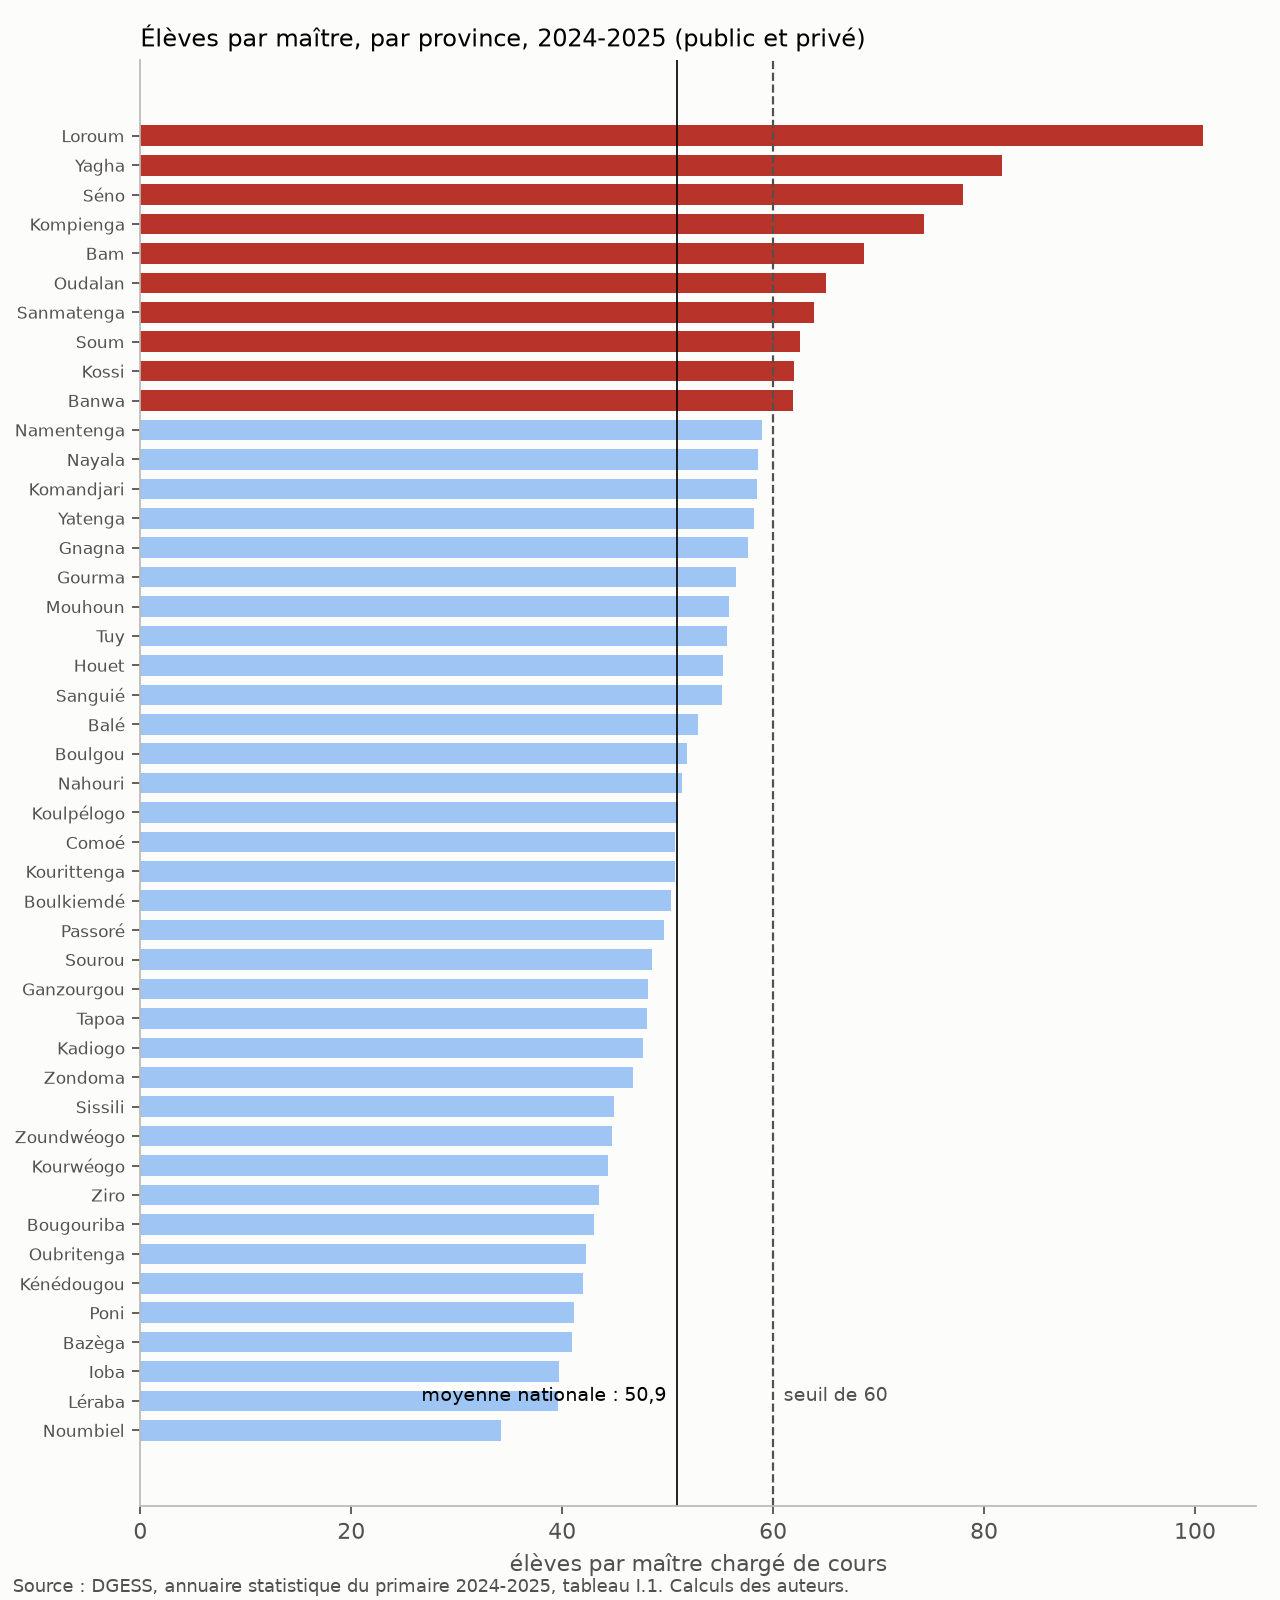
\includegraphics[width=\columnwidth]{fig_eleves_par_maitre.png}
\caption{Élèves par maître chargé de cours, par province, 2024-2025. En rouge : provinces au-delà de 60. Source : DGESS, annuaire du primaire 2024-2025, tableau I.1 ; calculs des auteurs.}
\label{fig:ratio}
\end{figure}

\subsection{La base Boussole}

La base est un fichier SQLite unique, dont chaque table est aussi exportée en CSV. Elle contient les trois tables de territoires, les huit tables de faits, un journal des rapprochements, un journal des lignes signalées, les résultats des contrôles et deux tables de métadonnées : \texttt{\_tables} décrit chaque table (contenu, grain, clé, sources, nombre de lignes) et \texttt{\_variables} est le dictionnaire des 159 variables (type, unité, description).

%======================================================================
\section{Contrôles}
%======================================================================

Les contrôles sont rejoués à chaque exécution (tableau~\ref{tab:controles}). Ils répondent aux consignes du challenge : vérifier les totaux contre les publications d'origine et se méfier des découpages et des noms~\cite{dcb_document}.

\begin{table*}[!t]
\centering
\small
\begin{tabularx}{\textwidth}{@{}L{5.6cm} Y L{1.6cm}@{}}
\toprule
Contrôle & Résultat & Statut \\
\midrule
45 provinces par édition & 45 pour chaque édition, sauf la Komandjari en 2022-2023, absente parce qu'aucune de ses écoles n'était ouverte & Conforme \\
Public + privé = total & Aucun écart sur les cinq variables & Conforme \\
Somme des provinces = total régional publié & Aucun écart sur 312 combinaisons édition, région et statut & Conforme \\
Élèves par maître recalculés = ratios publiés & Écart médian de 0,02 ; aucun écart supérieur à 0,1 sur 1\,071 lignes & Conforme \\
Salles : tableau de l'état des salles = tableau principal & Identiques dans 1\,020 cas sur 1\,077 ; écart médian de 2 salles dans les autres & Conforme, à noter \\
Effectifs : 45 provinces par année & 45 pour chacune des huit années & Conforme \\
Effectifs : garçons + filles = total & Aucun écart sur 2\,520 lignes & Conforme \\
Élèves par classe = élèves du tableau principal & Identiques pour les 359 provinces et années comparées & Conforme \\
Enseignants : somme des corps et des fonctions = total & Aucun écart sur 4\,239 lignes & Conforme \\
Enseignants tenant une classe = maîtres du tableau principal & Identiques dans 1\,077 cas sur 1\,077 & Conforme \
Projections : 45 provinces, 13 régions, 16 années & Complet, de 2020 à 2035 & Conforme \
Projections : hommes + femmes = ensemble & Aucun écart après interpolation des 24 valeurs décalées & Conforme \
Projections : somme des provinces = région & 20 écarts de plus de 5 personnes sur 4\,784 comparaisons & Conforme, à noter \\
Communes : couverture par région & 10 régions publiées sur 10 lues ; 85 à 100\,\% des communes, 69\,\% au Sahel & Conforme \\
Communes : somme des élèves = élèves de la province (DGESS) & Écart relatif médian nul sur 122 provinces et années complètes & Conforme \\
ESU : somme des provinces = total primaire publié & 18 tableaux fiables sur 40 (novembre 2021 à mai 2022, octobre 2023) & Conforme, à noter \\
ESU : filles + garçons = élèves touchés & 19 lignes incohérentes sur 420, toutes dans des rapports lus par reconnaissance de caractères & Conforme \\
Déplacés : aucune date perdue faute de P-code & 326 communes, 46 dates, de janvier 2019 à mars 2023 & Conforme \\
Métadonnées complètes & Toutes les tables et variables sont décrites & Conforme \\
\bottomrule
\end{tabularx}
\caption{Contrôles automatiques de la base \sol{}. Source : calculs des auteurs.}
\label{tab:controles}
\end{table*}

%======================================================================
\section{Limites et suite}
%======================================================================

Aucune donnée n'est disponible au niveau de l'école, ni sur les enseignants pris individuellement : le diagnostic descend à la province et, pour dix régions sur treize, à la commune. Les départs d'enseignants, les postes ouverts et les coûts unitaires des constructions ne figurent pas dans les données remises ; ils seront traités comme des hypothèses explicites dans le simulateur. Les chiffres de l'annuaire mêlent public et privé ; seul le public relève de l'affectation, et la base conserve les deux statuts séparément.

Le nettoyage est complet pour les sources retenues. L'étape suivante réunira ces tables dans une table d'analyse unique, par province et par année, qui alimentera la prévision de la demande et l'optimisation de la répartition.

%======================================================================
\section{Reproduction}
%======================================================================

La chaîne se relance depuis le dossier du projet, rangé dans le dossier des données des organisateurs, avec Python 3.11 ou plus récent et les bibliothèques de \texttt{requirements.txt}. La commande \texttt{python -m boussole.collecte} produit les copies brutes et le dépôt 01 ; \texttt{python -m boussole.nettoyage} construit la base, rejoue les contrôles et produit le dépôt 02. Les notebooks \texttt{01\_collecte} et \texttt{02\_nettoyage} présentent les mêmes étapes avec leurs résultats.

\textbf{Usage d'outils d'intelligence artificielle.} Conformément au règlement~\cite{dcb_document}, un assistant de programmation a été utilisé pour écrire et relire le code de la chaîne de traitement. Les données traitées sont des statistiques publiques agrégées ; aucune donnée personnelle n'a été manipulée. Chaque résultat a été vérifié par les contrôles décrits ci-dessus et relu par l'équipe.

\bibliographystyle{named}
\bibliography{references}

\end{document}
